\documentclass[journal = jacsat, manuscript = suppinfo]{achemso}

\usepackage[version = 4]{mhchem}
\usepackage{graphicx}
\usepackage{mwe}

% disable symbol next to email
\makeatletter
\def\acs@author@fnsymbol#1{}
\makeatother

\SectionNumbersOn

% macros
\newcommand{\nidppe}{\ce{Ni(dppe)Cl2}}
\newcommand{\nicl}{\ce{NiCl2 $\cdot$ 6H2O}}
\newcommand{\nh}{\ce{NH3}}
\newcommand{\nanh}{\ce{Na $\cdot$ NH3}}
\newcommand{\nhbr}{\ce{NH4Br}}
\newcommand{\h}{$^1$H}
\newcommand{\p}{$^{31}$P}
\newcommand{\cdcl}{\ce{CDCl3}}
\newcommand{\del}{$\delta = $}
\newcommand{\niion}{\ce{Ni^{2+}}}
\newcommand{\wavenum}{cm$^{-1}$}

\title{1,2-bis(diphenylphosphino)ethane (dppe) and \nidppe\ synthesis via
solvated electron reduction}

\author{David Qiu}
\affiliation{Department of Chemistry, University of Illinois at
Urbana-Champaign, 505 S Matthews Avenue, Urbana, IL, 61801}
\email{davidlq2@illinois.edu}

\begin{document}

\tableofcontents

\section{General Considerations}

\h\ NMR spectra were taken on a 60 MHz Nanalysis NMReady-60PRO tabletop NMR
instrument coupled with a STC-1000 digital temperature controller. \p\ NMR
spectra were taken on a 400 MHz  Varian NMR spectrometer. IR spectra were taken
on a Perkin Elmder Spectrum Two FTIR spectrometer.

n-hexane, ethanol, and \nh\ were sourced from UIUC. Diethyl ether, Na were
sourced from Fischer Chem. 1,2-dichloroethane, triphenylphosphine were sourced
from Acros. \nhbr\ was sourced from Oakwood Chemical.

\section{Experimental Procedures}

\textbf{dppe synthesis\cite{handout}:} To a round bottom flask was charged 200
mL of \nh, a glass-coated stir bar, and a dry ice condenser. Na (2.379 g, 0.1035
mol, 4 equiv.) was added slowly over 3 minutes. A dark blue solution was allowed
to form over 10 minutes, and then triphenylphosphine (13.55 g, 0.05166 mol, 2
equiv.) was added in 1 g portions.  This solution reacted for 30 minutes, after
which \nhbr\ (5.068 g, 0.05174 mol, 2 equiv.) was added. 1,2-dichloroethane
(2.555 g, 0.02582 mol, 1 equiv.) was poured in and reacted for 10 minutes.  The
flask was left open to air for 1 week.

The dried dppe was washed with DI water and rotary evaporated following
dilution with ethanol. The purified dppe crystals then precipitated, and were
filtered out of solution and washed with ethanol.

\textbf{\nidppe\ synthesis\cite{handout}:} \nicl\ (0.320 g, 1.34 mol, 1 equiv.)
was dissolved in ethanol and mixed with dppe (0.54 g, 1.34 mol, 1 equiv.). This
was allowed to react for 5 minutes, forming a tomato-red solution.  \nidppe\ was
filtered out and washed with diethyl ether. \h, \p\ NMR and IR spectra were
taken of dppe and \nidppe, and are available for viewing in the Supporting
Information.

\textbf{\h\ and \p\ NMR:} \h\ and \p\ NMR were taken, and the results were as
follows. (*) denotes an unidentified impurity.

In the dppe NMR spectrum: \h: \del\ 7.27 ppm (20 H), \del\ 2.06 ppm (4
H, t), \del\ 3.58 ppm (diethyl ether \cite{nmrtable}, q), \del\ 1.21 ppm
(diethyl ether \cite{nmrtable}, t), \del\ 1.60 ppm (HDO \cite{nmrtable}, s).
\p: \del\ -11.52 ppm (dppe), \del\ -105.91 ppm (*), \del\ -221.00 ppm (*).

In the \nidppe\ NMR spectrum: \h: \del\ 8.01 ppm (16 H), \del\ 7.53 ppm (24 H),
\del\ 7.24 ppm (\cdcl), \del\ 2.12 ppm (8 H), \del\ 1.50 ppm (HDO). \p
\p: \del\ 58.23 ppm (\nidppe), \del\ -105.91 ppm (*), \del\ -221.00 ppm (*).

In the dppe IR spectrum: $\nu$ = 3300 \wavenum\ (O-H), $\nu$ = 2950 \wavenum\
(C-H).


\section{NMR and IR Spectra}

\begin{figure}[H]
	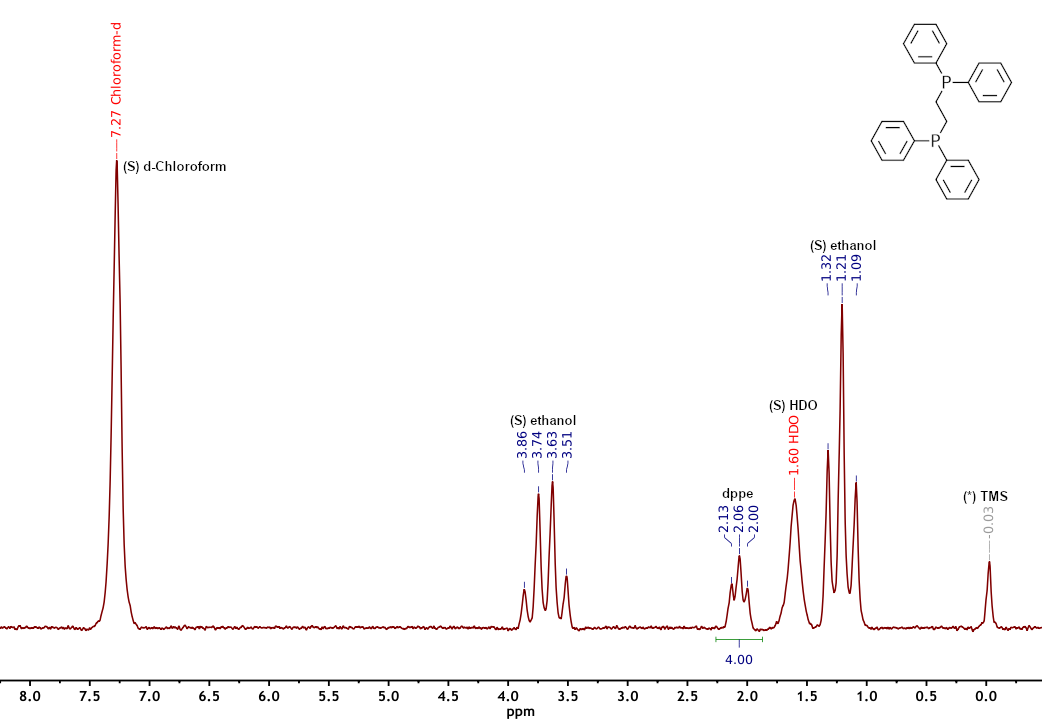
\includegraphics[width=\textwidth]{figures/dppe_hnmr}
	\caption{\h\ NMR spectrum of dppe.}
\end{figure}
\begin{figure}[H]
	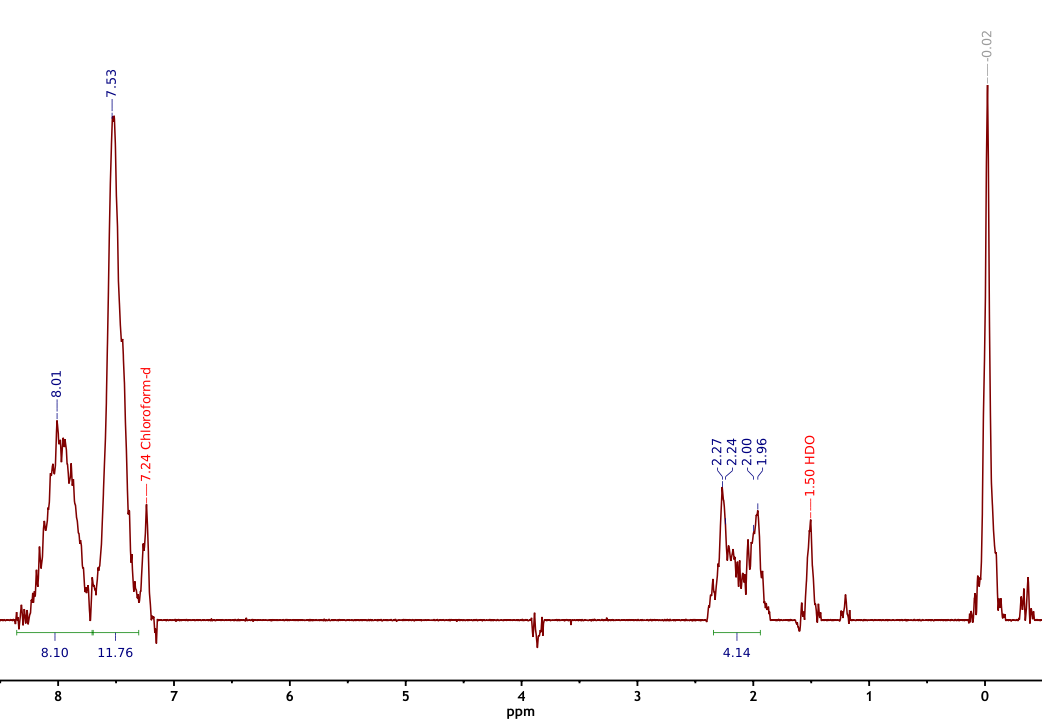
\includegraphics[width=\textwidth]{figures/nidppe_hnmr.png}
	\caption{\h\ NMR spectrum of \nidppe.}
\end{figure}
\begin{figure}[H]
	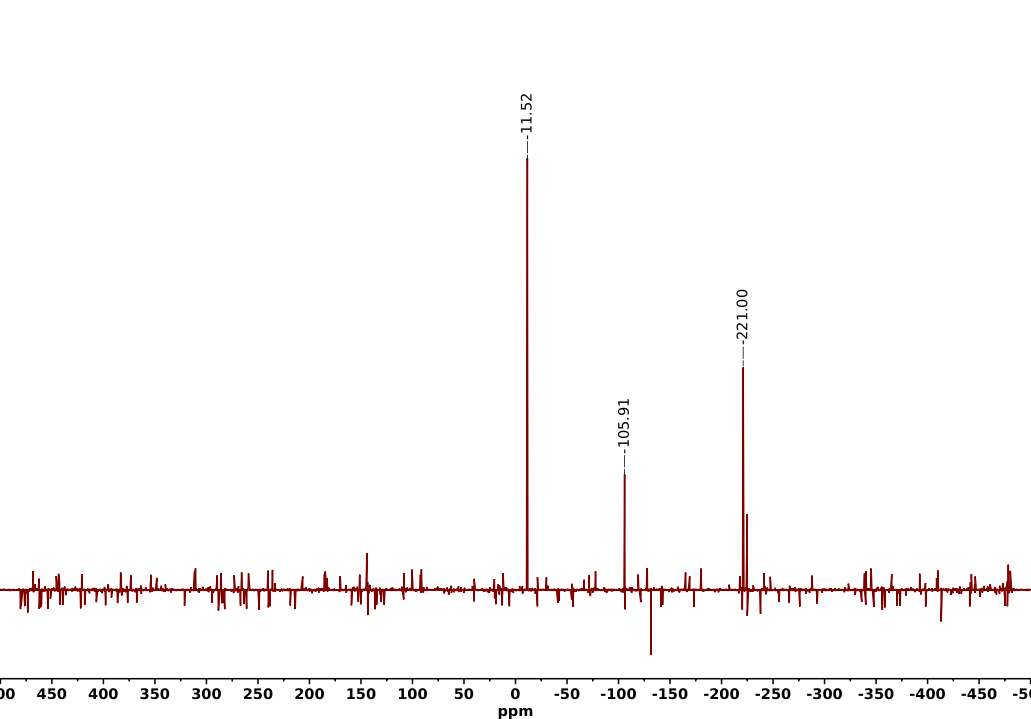
\includegraphics[width=\textwidth]{figures/dppe_pnmr.png}
	\caption{\p\ NMR spectrum of dppe.}
\end{figure}
\begin{figure}[H]
	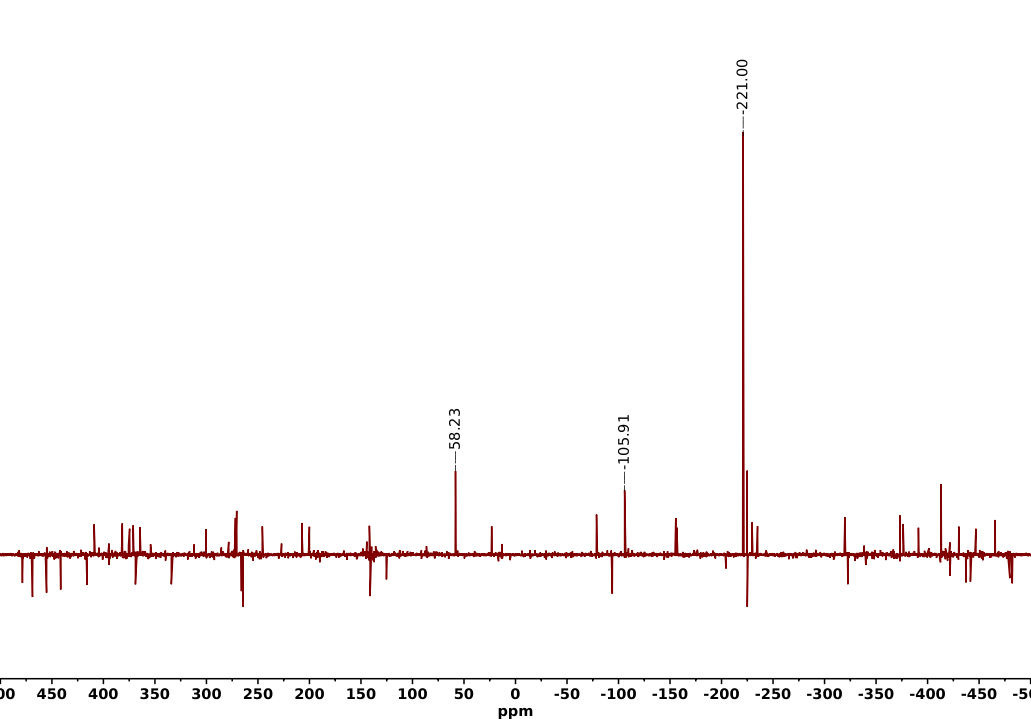
\includegraphics[width=\textwidth]{figures/nidppe_pnmr.png}
	\caption{\p\ NMR spectrum of \nidppe.}
\end{figure}
\begin{figure}[H]
	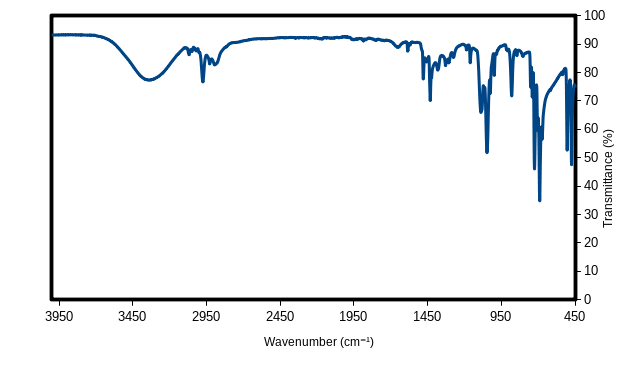
\includegraphics[width=\textwidth]{figures/dppe_ir.png}
	\caption{IR spectrum of dppe.}
\end{figure}
\begin{figure}[H]
	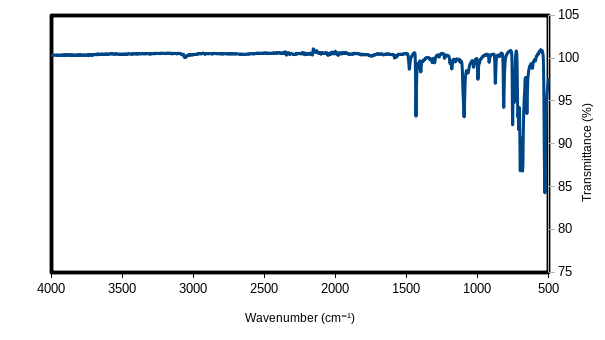
\includegraphics[width=\textwidth]{figures/nidppe_ir.png}
	\caption{IR spectrum of \nidppe.}
\end{figure}

\bibliography{lab_3.bib}

\end{document}
